\chapter{ĐÁNH GIÁ VÀ KẾT LUẬN}
\begin{flushleft}
	\fontsize{12pt}{7pt}\selectfont
	\textit{Chương này sẽ đánh giá chi tiết về kết quả thực hiện hai chức năng của đề tài. Tiếp theo sẽ đánh giá về tiến độ thực hiện so với kế hoạch thực hiện đã đề ra ban đầu. Cuối cùng là trình bày về các hướng phát triển trong tương lai của đề tài.}
\end{flushleft}

\section{Đánh giá kết quả đề tài}

	Kết quả luận văn này nhóm sẽ đánh giá dựa trên hai tiêu chí. Tiêu chí thứ nhất là đánh giá kết quả so với các mục tiêu mà nhóm đề ra trong luận văn này. Tiêu chí thứ hai là đánh giá kết quả thực hiện so với tiến độ thực hiện mà nhóm đề xuất trong giai đoạn Đề Cương Luận Văn Tốt Nghiệp.
	
\subsection{Đánh giá so với các mục tiêu đề ra}

	Với mục tiêu sinh mã điều khiển có điều kiện theo chuẩn SCORM, nhóm đã hiện thực thành công một số trường hợp thông dụng đối với người học. SCORM Engine của SCORM Cloud đã nhận được các thông tin điều khiển có điều kiện mà nhóm sinh ra trong file imsmanifest.xml và hoạt động tốt. Mặc dù chưa tiến hành thu thập ý kiến của người sử dụng để có được thêm nhiều trường hợp điều khiển hơn. Thử nghiệm thực tế cho thấy chức năng này hoạt động tương đối tốt với các hệ quản trị đào tạo có SCORM Engine được hỗ trợ chức năng điều khiển có điều kiện theo chuẩn SCORM.\\
	
	Với mục tiêu hiện thực chức năng tổng hợp bài kiểm tra, SCORM Engine đã nhận được thông tin về nội dung của các câu hỏi được chọn. Khi người học tiếp cận nội dung, các câu hỏi được người biên soạn lựa chọn sẽ được hiển thị ngẫu nhiên. Kết quả thực tế cho thấy chức năng này hoạt động tốt nhưng còn hạn chế là chỉ có một loại câu hỏi dạng nhiều lựa chọn với một đáp án đúng, do đó loại câu hỏi chưa đa dạng.
	
\newpage
\subsection{Đánh giá so với tiến độ đề ra}

\begin{center}
	\begin{figure}[htp]
		\begin{center}
			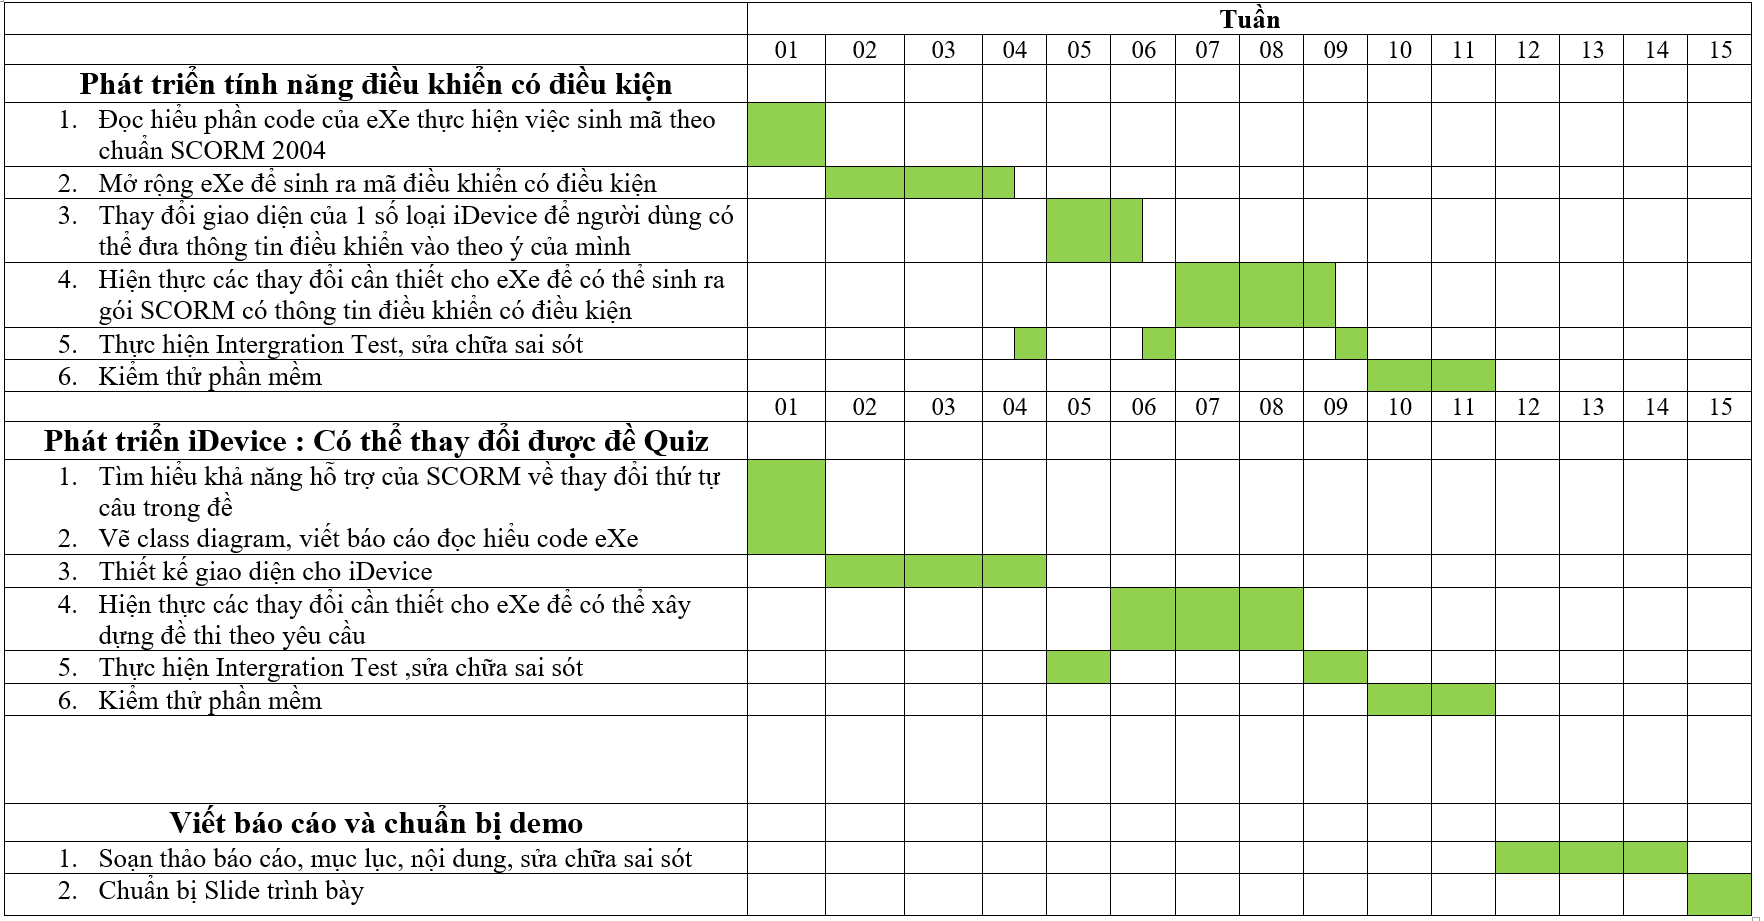
\includegraphics[width=13cm]{Chapter6/Pictures/picture61.png}
		\end{center}
		\caption{Kế hoạch đã đề ra}
		\label{refhinhchuong7xx11}
	\end{figure}
\end{center}

	Trong giai đoạn Đề Cương Luận Văn Tốt Nghiệp, nhóm đã đề xuất kế hoạch thực hiện như hình 6.1. Kế hoạch đề xuất để thực hiện Luận Văn Tốt Nghiệp bao gồm mười lăm tuần, trong đó ba nhóm công việc chính là phát triển tính năng điều khiển có điều kiện, phát triển công cụ tạo bài kiểm tra và viết báo cáo Luận Văn Tốt Nghiệp.\\
	
	Tuy nhiên so với kết quả thực tế, do gặp phải một số khó khăn trong việc tìm hiểu công nghệ bên trong hệ thống nên thời gian trên đã bị thay đổi. Ban đầu trong kế hoạch đề ra, nhóm sẽ thực hiện hai nhóm công việc là phát triển chức năng điều khiển có điều kiện và chức năng phát triển công cụ có khả năng tổng hợp câu hỏi, tạo đề kiểm tra song song với nhau. Nhưng việc chia nhiệm vụ như thế dẫn đến việc các thành viên hoạt động không tập trung và gây mất hiệu quả. Do đó nhóm quyết định tập trung phát triển từng chức năng một. Sau đây là kế hoạch thực hiện theo thực tế.
	
	\begin{center}
		\begin{figure}[htp]
			\begin{center}
				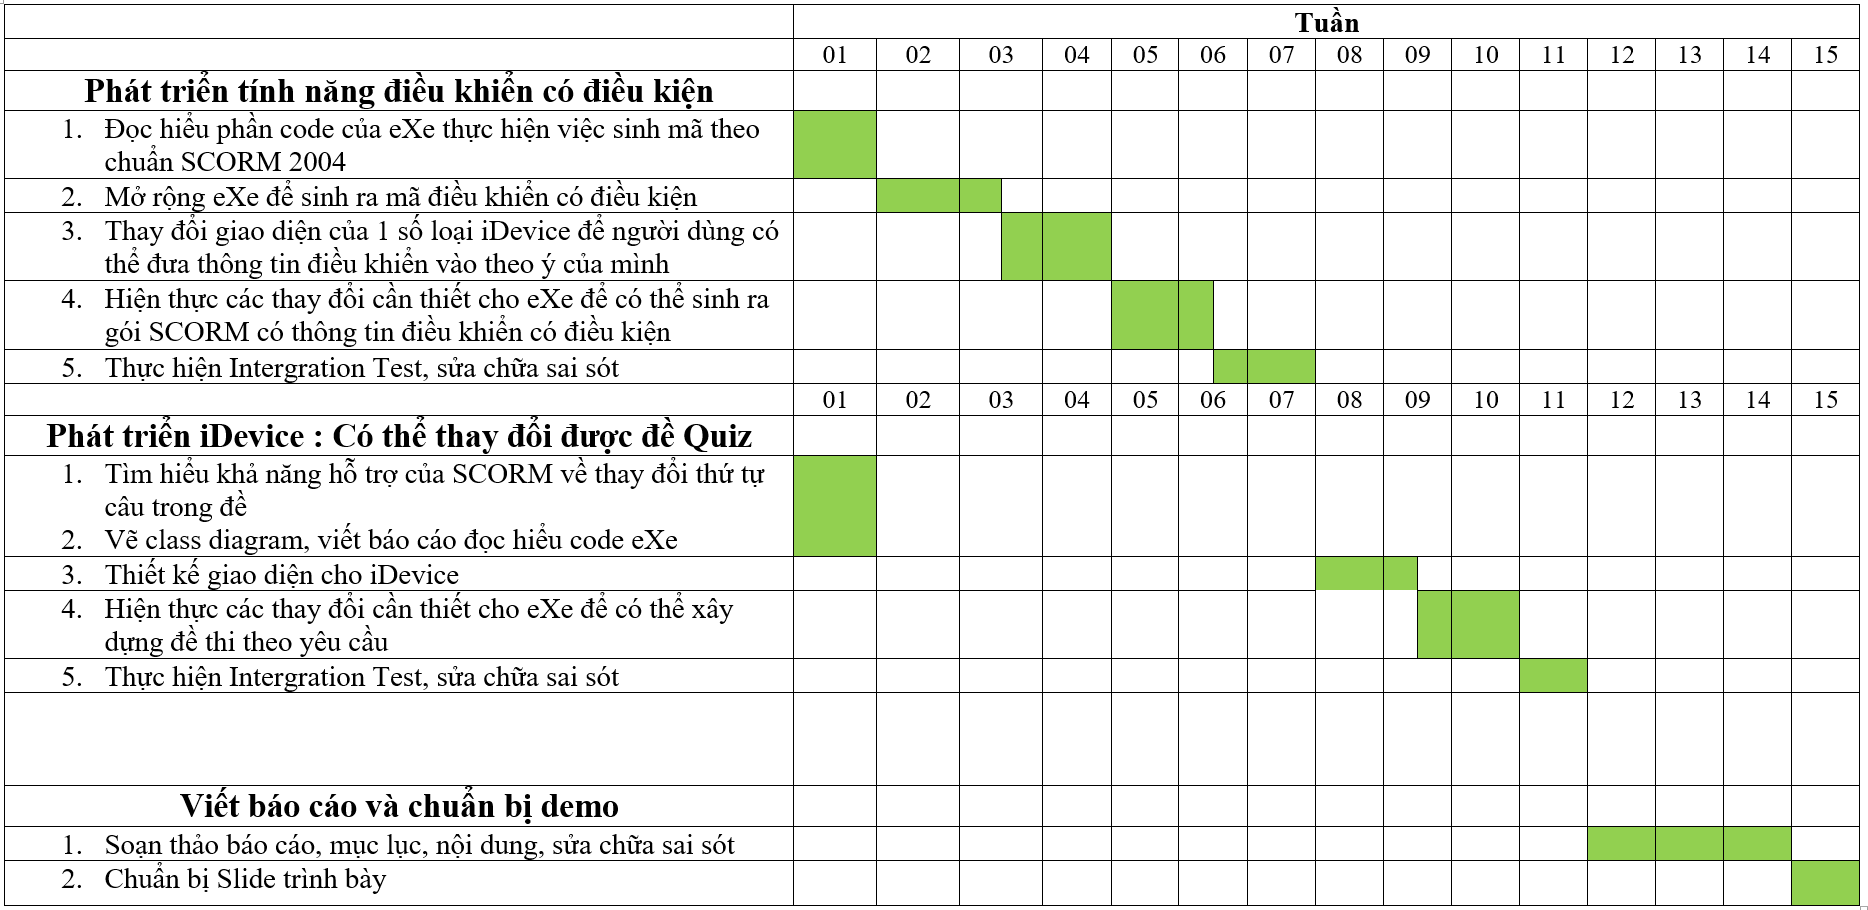
\includegraphics[width=13cm]{Chapter6/Pictures/picture62.png}
			\end{center}
			\caption{Kế hoạch thực hiện theo thực tế}
			\label{refhinhchuong7xx11}
		\end{figure}
	\end{center}
	
	\newpage
	
	
	Hình 6.2 thể hiện kế hoạch thực tế do nhóm thực hiện. Nhóm tập trung hiện thực chức năng đầu tiên là phát triển chức năng điều khiển có điều kiện theo chuẩn SCORM trước, sau khi hoàn thành chức năng này thì nhóm tập trung phát triển chức năng thứ hai là phát triển công cụ tổng hợp câu hỏi và tạo bài kiểm tra.
	
\section{Các hướng phát triển sau này}

Với những kết quả đánh giá sau khi thực hiện hoàn tất Luận Văn Tốt Nghiệp này, nhóm đề xuất một số hướng phát triển có thể hiện thực trong tương lai:
	\begin{itemize}
		\item Thứ nhất, từ khung kiến trúc hệ thống của eXe Learning, giao diện có thể được hiện thực lại bằng các công nghệ mới hơn hiện nay như ReactJS và phần hệ thống có thể phát triển bằng NodeJS hoặc Django.
		
		\item Thứ hai là cần phải nghiên cứu các phản hồi từ phía người dùng để cải tiến thêm một số chức năng điều khiển có điều kiện, thêm vào một số loại câu hỏi khác nhau như điền vào chỗ trống, True/False Questions,...
	\end{itemize}

\begin{comment}
\newpage

\begin{center}

	\LARGE{\textit{Tóm tắt nội dung}}\\
	\Large{\textbf{Mở rộng chức năng cho một hệ thống\\ hỗ trợ xây dựng dữ liệu theo chuẩn SCORM}}
\end{center}
\vspace{1cm}

	Trong đề tài Luận Văn Tốt Nghiệp này, nhóm nghiên cứu và mở rộng chức năng cho công cụ eXe Learning, một công cụ hỗ trợ soạn thảo nội dung bài học trực tuyến và xuất dữ liệu theo chuẩn SCORM. eXe Learning là một công cụ mã nguồn mở, ra đời với mục đích hỗ trợ việc soạn thảo bài học trực tuyến. Nhóm đề xuất mở rộng và hiện thực hai chức năng cho eXe để phục vụ tốt hơn cho việc soạn thảo.\\
	
	Chức năng thứ nhất là chức năng thiết lập điều khiển có điều kiện cho các bài học trong một khóa học. Chức năng này giúp cho người soạn thảo có thể thiết lập được trình tự cho các bài học trong một khóa học, giúp người học có một lộ trình học hợp lý.\\
	
	Chức năng thứ hai là phát triển một công cụ có thể tổng hợp câu hỏi và tạo bài kiểm tra. Hiện tại eXe Learning có hỗ trợ công cụ kiểm tra, tuy nhiên tính năng của nó còn một số hạn chế, vì vậy cần có một công cụ kiểm tra mạnh hơn, có thể tổng hợp câu hỏi với nhiều mức độ khác nhau, đặc biệt công cụ này có thể tự động sinh bài kiểm tra có vị trí các câu hỏi cũng như các câu trả lời thay đổi ở mỗi lần thực hiện.

\vspace{2cm}

	\begin{center}
		\LARGE{\textit{Abstract}}\\
		\Large{\textbf{Extend features for an Authoring tool supported SCORM}}
	\end{center}
\vspace{1cm}

In this thesis, we study and extend the feature of the eXe Learning tool, which have editing and SCORM support. eXe Learning is an open source tool, created for the purpose of supporting online learning. We propose to extend and implement two features for eXe to better serve the editing. \\

The first feature is the conditional control setting function for the lessons in a course. This function allows the teacher to set the sequence for the lessons in a course, giving the learner a reasonable learning procedure.

The second feature is to develop a tool that can synthesize questions and create tests. Currently, eXe Learning has support for testing tools, but its features are limited, so there needs to be a more powerful testing tool that can synthesize questions into many different levels. This tool can automatically generate quizzes that place the questions as well as the answer changes at each execution.

\end{comment}

\newpage

	\begin{thebibliography}{9}
	
\bibitem{}
UK eUniversities Worldwide, November 2002. 
\textbf{“Principles and practice in E-Learning platform architecture”}.
\textit{\href{www.ukeu.com.}{www.ukeu.com.}}.

\bibitem{}
Xiaofei Liu, Abdulmotaleb El Saddik, Nicolas D. Georganas. Đại học Ottawa, Ontario, Canada,
\textbf{“An Implementable Architecture of an E-Learning System”}.
\textit{\href{www.Ott.edu.ca}{www.Ott.edu.ca}}.

\bibitem{}
About Sequencing and Navigation of SCORM 2004: \textbf{“SCORM Technical”}. \textit{\href{https://scorm.com/scorm-explained/technical-scorm/sequencing/}{https://scorm.com/scorm-explained/technical-scorm/sequencing/}}.

\bibitem{}
Twisted Framework: Document of Twisted and How to use to build url dispatch
\textbf{“Twisted Framework Introduction”}.
\textit{\href{https://twistedmatrix.com/documents/12.3.0/web/howto/web-in-60/dynamic-dispatch.html}{https://twistedmatrix.com/documents/12.3.0/web/howto/web-in-60/dynamic-dispatch.html}}	

\bibitem{}
Nevow Framework: Document of Nevow on Github - Construction Kit
\textbf{“Nevow Document”}.
\textit{\href{https://github.com/twisted/nevow}{https://github.com/twisted/nevow}}	

\bibitem{}
ExtJS Tutorial: ExtJS-Tutorial.com
\textbf{“Introduction ExtJS”}.
\textit{\href{https://www.extjs-tutorial.com}{https://www.extjs-tutorial.com}}.

%7
\bibitem{}
Tutorial Spoint - Tutorial Spoint: Learn ExtJS Basic via Example
\textbf{“ExtJS Tutorial”}.
\textit{\href{https://www.tutorialspoint.com/extjs/index.htm}{https://www.tutorialspoint.com/extjs/index.htm}}.
	
%8	
\bibitem{}
Client-server - What is Client-server and software architecture model consisting of two parts
\textbf{“Client-server software architecture”}.
\textit{\href{https://simple.wikipedia.org/wiki/Client-server}{https://simple.wikipedia.org/wiki/Client-server}}.

%9
\bibitem{}
eXeLearning - Documentation, Tutorial and How to Install
\textbf{“eXeLearning Documentation”}.
\textit{\href{https://simple.wikipedia.org/wiki/Client-server}{https://simple.wikipedia.org/wiki/Client-server}}

%10
\bibitem{}
eXeLearning - Wikipedia, The eXeLearning Development Team
\textbf{“eXeLearning Wikipedia”}.
\textit{\href{https://simple.wikipedia.org/wiki/Client-server}{https://simple.wikipedia.org/wiki/Client-server}}


%11
\bibitem{}
Selenium - What is Selenium and Selenium automates browsers
\textbf{“Selenium Project”}.
\textit{\href{https://www.seleniumhq.org/}{https://www.seleniumhq.org/}}


\bibitem{}
Selenium WebDriver: Overview and How to use Selenium WebDriver
\textbf{“Selenium WebDriver: Overview”}.
\textit{\href{https://viblo.asia/p/selenium-webdriver-part-1-WAyK8x8EKxX}{https://viblo.asia/p/selenium-webdriver-part-1-WAyK8x8EKxX}}.

\end{thebibliography}


